\documentclass[12pt]{article}

% packages

%\usepackage{times} % alt: cmbright
\usepackage[top=1in, bottom=1in, left=1in, right=1in]{geometry}
\usepackage{natbib}
\usepackage{amsmath}
\usepackage{amssymb}
\usepackage{latexsym}
\usepackage{sectsty}
\usepackage{amsfonts}
\usepackage{epsfig}
\usepackage{url}
\usepackage{microtype}
\usepackage{fixmath}
\usepackage{hyperref}
\usepackage{amsthm}
\usepackage{subfigure}
\usepackage{float}
\usepackage{hyperref}

\newtheorem{lem}{Lemma}
\newtheorem{defn}{Assumption}
\newtheorem{propty}{Property}
\newtheorem{thm}{Theorem}

% references

\newcommand{\mysec}[1]{Section~\ref{sec:#1}}
\newcommand{\myapp}[1]{Appendix~\ref{app:#1}}
\newcommand{\myeq}[1]{Equation~\ref{eq:#1}}
\newcommand{\myeqp}[1]{Eq.~\ref{eq:#1}}
\newcommand{\mychap}[1]{Chapter~\ref{chap:#1}}
\newcommand{\myfig}[1]{Figure~\ref{fig:#1}}

% math conveniences

\newcommand{\g}{\,\vert\,}
\newcommand{\E}{\textrm{E}}
\newcommand{\vct}[1]{\textbf{#1}}
\newcommand{\realline}{\mathbb{R}}
\newcommand{\indpt}{\protect\mathpalette{\protect\independenT}{\perp}}
\def\independenT#1#2{\mathrel{\rlap{$#1#2$}\mkern2mu{#1#2}}}
\newcommand{\h}[1]{\textrm{H}\left( #1 \right)}
\newcommand{\half}{\frac{1}{2}}
\newcommand{\new}{\textrm{new}}

\newcommand{\mult}{\textrm{Mult}}
\newcommand{\dir}{\textrm{Dir}}
\newcommand{\discrete}{\textrm{Discrete}}
\newcommand{\Bern}{\textrm{Bern}}
\newcommand{\DP}{\textrm{DP}}
\newcommand{\GP}{\textrm{GP}}
\newcommand{\Bet}{\textrm{Beta}}

% paragraph spacing

\setlength{\parindent}{0pt}
\setlength{\parskip}{2ex plus 0.5ex minus 0.2ex}

\allsectionsfont{\sffamily\mdseries}
\paragraphfont{\sffamily\bfseries}

\usepackage{algorithm}
\usepackage{algorithmic}
\renewcommand{\algorithmicrequire}{\textbf{Input:}}
\renewcommand{\algorithmicensure}{\textbf{Output:}}


\begin{document}

\title{\textsf{Greedy maximization of submodular functions}}
\author{\textsf{Daqing Yi}}
\date{\textsf{CS611 Assignment 1}}

\maketitle

%\section{Requirement}
%\begin{itemize}
%\item (numbered) definitions for every concept in the theorem statement 
%\item provide at least one figure and one simple example
%\item provide some explanation of why the theorem is interesting/important and to what situations it applies 
%\item provide a logic-and-proof-strategies analysis of the theorem's proof
%\end{itemize}


The theorem to be proved in this paper is from \cite{krause2012submodular}.

\section{Definitions}

\begin{mydef}[\textbf{Set Function}]
\label{def:sef_func}
Functions $ f: 2^{V} \rightarrow \mathbb{R} $ that assign each subset $ S \subseteq V $ a value $ f(S) $, in which $ V $ is a finite set, commonly called the \emph{ground set}.
\end{mydef}

\begin{mydef}[\textbf{Discrete Derivative}]
\label{def:dis_der}
For a set function $ f: 2^{V} \rightarrow \mathbb{R} $, $ S \subseteq V $, and $ e \in V $, let $ \Delta_{f}(e|S):= f(S \cup \{e\}) - f(S) $ be the \emph{discrete derivative} of $ f $ at $ S $ with respect to $ e $. 
\end{mydef}

For short, let $ \Delta(e|S) = \Delta_{f}(e|S) $.

\begin{mydef}[\textbf{Submodularity}]
\label{def:submodular}
A function $ f: 2^{V} \rightarrow \mathbb{R} $ is \emph{submodular} if for every $ A \subseteq B \subseteq V $ and $ e\in V \setminus B $ it holds that
\begin{center}
$ \Delta(e | A ) \geq \Delta(e | B) $.
\end{center}

Equivalent, a function $ f: 2^{V} \rightarrow \mathbb{R} $ is \emph{submodular} if for every $ A, B \subseteq V $,
\begin{center}
$ f(A \cap B) + f(A \cup B) \leq f(A) + f(B) $.
\end{center}
\end{mydef}

Submodularity is an intuitive diminishing returns property, stating that adding an element to a smaller set helps more than adding it to a larger set. 

Fig. \ref{fig:Submodular} gives an example on diminishing returns effect on submodular problem, which is placing sensors in a water distribution network to detect contaminations. When adding a new sensor $ s' $ (red region), if more sensors are already placed (b), there is more overlap, hence less gain in utility: $ \Delta( s' \mid \{s_{1}, s_{2} \} ) \geq \Delta ( s' \mid \{ s_{1}, \cdots , s_{4} \} ) $ .

\begin{figure}[H]
\centering
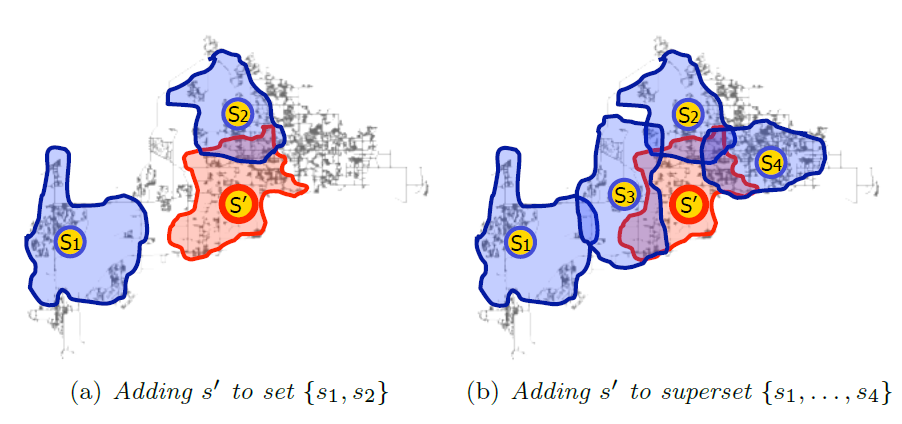
\includegraphics[width=0.7\linewidth]{./Submodular}
\caption{An example of submodularity}
\label{fig:Submodular}
\end{figure}


\begin{mydef}[\textbf{Monotonicity}]
A function $ f: 2^{V} \rightarrow \mathbb{R} $ is \emph{monotone} if for every $ A \subseteq B \subseteq V, f(A) \leq f(B) $.
\end{mydef}

A function $ f $ is monotone iff all its discrete derivatives are nonnegative, which is 
$ \forall A \subseteq V $ and $ e \in V $, $ \Delta (e|A) \geq 0 $.

\begin{figure}[H]
\centering
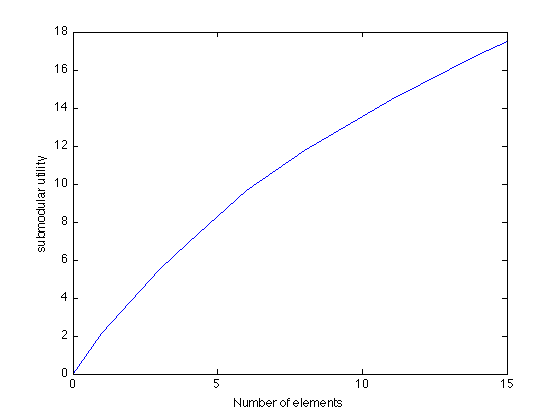
\includegraphics[width=0.45\linewidth]{./monotone}
\caption{An example of monotonicity}
\label{fig:monotone}
\end{figure}

Submodular functions have properties which are very similar to convex and concave functions. Here we focus on the problem of maximizing a submodular function subject to some constraints.

\begin{mydef}[\textbf{Maximization of submodular function}]

Let $ f : 2^{V} \rightarrow \mathbb{R} $ be submodular function, 

\begin{center}
 $ \max_{S \subseteq V} f(S) $; \\
 subject to some constraint on $ S  $.

\end{center}
\end{mydef}

%Before stating the theorem, we also need a Lemma to support the proof, which is omitted in original paper \cite{krause2012submodular}.
%\begin{lem}
%\label{lem:submod}
%If a set function $ f : 2^{V} \rightarrow \mathbb{R} $ is monotonic submodular, for $ S \subseteq V $ and $ e \in V $, $ \Delta(e|S) $ defined in Definition \ref{def:dis_der} is also monotomic submodular.
%\begin{proof}
%[TODO: add proof]
%\end{proof}
%\end{lem}

\section{Theorem}

Here we are interested with one of the constraints, cardinailty constraint, in which we require that $ | S | \leq k $. It is very commonly used in applications with the limitations on the number of planning steps.
\begin{mydef}[\textbf{Maximization of submodular function with cardinality constraint}]
\begin{center}
$ \max_{S \subseteq V} f(S),  | S | \leq k $
\end{center}
\end{mydef}

For many classes of submodular functions, this problem has been proved to be NP-hard. An efficient algorithm with theoretical approximation guarantee is expected. The \emph{greedy algorithm} is mentioned.

\begin{mydef}[\textbf{The greedy algorithm}]
Start with the empty set $ S_{0} $,
in iteration $ i $,
add the element maximizing the discrete $ \Delta(e \mid S_{i-1}) $:
\begin{equation}
\label{eq:greedy}
S_{i} = S_{i-1} \cup \{ \arg \max_{e} \Delta(e \mid S_{i-1}) \}
\end{equation}

\end{mydef}

In \cite{nemhauser1978analysis}, it is proved that the greedy algorithm provides a good approximation to the optimal solution of the NP-hard optimization problem.

\begin{thm} 
\label{thm:submax}
(\cite{nemhauser1978analysis}) Fix a nonnegative monotone submodular function $ f : 2^{V} \rightarrow \mathbb{R}_{+} $ and let $ {\{S_{i}\}}_{i\geq0} $ be the greedily selected sets defined in Eq.(\ref{eq:greedy}). Then for all positive integers $ k $ and $ l $, 
\begin{center}
$ f(s_{l}) \geq (1-e^{-l/k}) \max_{S:|S| \leq k} f(S) $.
\end{center}
In particular, for $ l = k, f(S_{k}) \geq (1-1/e) \max_{|S| \leq k} f(S) $.
\end{thm}

\section{Proof}

The proof strategy is finding the performance guarantee at single step and then applying multiple steps.

Let's firstly fix $ l $ and $ k $. Due to monotonicity of $ f $, we can convert $ S^{*} \in \arg \max {f(S): |S| \leq k} $ to $ S^{*} \in \arg \max {f(S): |S| = k} $. Write it in the form of elements in set $ S^{*} $, which is $ S^{*} = \{ v^{*}_{1}, \cdots v^{*}_{k} \} $.

By monotonicity of $ f $, we have
\begin{equation}
\label{eq:monotonicity}
f(S^{*}) \leq f(S^{*} \cup S_{i}) 
\end{equation}

By telescoping sum , we have
\begin{equation}
\label{eq:teleSumDet}
\begin{aligned}
f(S^{*} \cup S_{i}) & = f(\{ v^{*}_{1}, \cdots , v^{*}_{k} \} \cup S_{i}) \\
& = f(S_{i}) + \Delta( \{ v^{*}_{1}, \cdots , v^{*}_{k} \} \mid S_{i} ) \\
& = f(S_{i}) + \Delta( v^{*}_{1} \mid S_{i} ) + f( \{ v^{*}_{2}, \cdots , v^{*}_{k} \} \mid S_{i} \cup \{ v^{*}_{1} \}  ) \\
& \cdots \\
& = f(S_{i}) + \sum_{j=1}^{k} \Delta(v^{*}_{j} \mid S_{i} \cup \{ v^{*}_{1}, \cdots , v^{*}_{j-1} \})
\end{aligned}
\end{equation}


%\begin{equation}
%\label{eq:teleSum}
%f(S^{*} \cup S_{i}) = f(S_{i}) + \sum_{j=1}^{k} \Delta(v^{*}_{j} \mid S_{i} \cup \{ v^{*}_[1], \cdots , v^{*}_{j-1} \})
%\end{equation}

By Definition \ref{def:submodular}, we can have $ \Delta(v^{*}_{j} \mid S_{i} \cup \{ v^{*}_{1}, \cdots , v^{*}_{j-1} \}) \leq \Delta(v^{*}_{j} \mid S_{i}) $, since $ S_{i} \subseteq S_{i} \cup \{ v^{*}_{1}, \cdots , v^{*}_{j-1} \} $. Applying to Eq.(\ref{eq:teleSumDet}) gets 
\begin{equation}
\label{eq:proofSubmodular}
%\begin{aligned}
f(S^{*} \cup S_{i}) \leq f(S_{i}) + \sum_{j=1}^{k} \Delta(v^{*}_{j} \mid S_{i} )
%\end{aligned}
\end{equation}

By modifying Eq.(\ref{eq:proofSubmodular}) to set notation from $ \sum_{j=1}^{k} \Delta(v^{*}_{j} \mid S_{i} ) $ to $ \sum_{v \in S^{*}} \Delta(v \mid S_{i}) $, we have
\begin{equation}
\label{eq:proofSubmodular2}
f(S^{*} \cup S_{i}) \leq f(S_{i}) + \sum_{v \in S^{*}} \Delta(v \mid S_{i}).
\end{equation}

Because ``greedy" means to choose the maximum at one step $ f(S_{i+1}) - f(S_{i}) \geq f( \{ v^{*}_{i+1} \} \cup S_{i} ) - f(S_{i}) = \Delta(v \mid S_{i}), v \in S^{*}  $  Apply to Eq.(\ref{eq:proofSubmodular2}) we have 
\begin{equation}
\label{eq:proofGreedy}
f(S^{*} \cup S_{i}) \leq f(S_{i}) + \sum_{v \in S^{*}} (f(S_{i+1}) - f(S_{i}))
\end{equation}

Notice here $ f(S_{i+1}) - f(S_{i}) $ in Eq.(\ref{eq:proofGreedy}) is independent with $ v $. As $ | S^{*} | \leq k  $ to Eq.(\ref{eq:proofGreedy}), we have
\begin{equation}
\label{eq:proofSizeLimit}
f(S^{*} \cup S_{i}) \leq f(S_{i}) + k(f(S_{i+1} - f(S_{i}))
\end{equation}

By applying Eq.(\ref{eq:proofSizeLimit}) to Eq.(\ref{eq:monotonicity}) and move $ f(S_{i}) $ to left-hand side, we can have
\begin{equation}
\label{eq:inequality}
f(S^{*}) - f(S_{i}) \leq k(f(S_{i+1}) - f(S+_{i}))
\end{equation}

Now define $ \delta_{i} = f(S^{*}) - f(S_{i}) $, we can also have $ \delta_{i} - \delta_{i+1} = f(S_{i+1}) - f(S+_{i}) $. Hence, Eq.(\ref{eq:inequality}) can be rewritten as $ \delta_{i} \leq k(\delta_{i} - \delta_{i+1}) $.

By arranging it, we have
\begin{equation}
\label{eq:singlePer}
\delta_{i+1} \leq (1 - \frac{1}{k})\delta_{i}.
\end{equation}

By applying Eq.(\ref{eq:singlePer}) $ l $ times to $ \delta_{0} $, we can have
\begin{equation}
\delta_{l} \leq (1-\frac{1}{k})^{l}\delta_{0}.
\end{equation}

Next note that $ \delta_{0} = f(S^{*} - f(\phi)) $ and let $ f(\phi) = 0 $. Then we have
\begin{equation}
\delta_{0} = f(S^{*}).
\end{equation}

For all $ x \in \mathbb{R} $, we have

\begin{equation}
\delta_{l} \leq (1 - \frac{1}{k})^{l} \delta_{0} = (1 - \frac{1}{k})^{l} f(S^{*}) \leq e^{- l/k} f(S^{*}).
\end{equation}

Substituting $ \delta_{l} = f(S^{*}) - f(S_{l}) $ and rearranging then yields the claimed bound of $ f(S_{l}) \geq (1-e^{-l/k})f(S^{*}) $.

Hence Theorem \ref{thm:submax} is proved.

\section{Applications}

Theorem \ref{thm:submax} shows that the greedy algorithm works on maximum optimization of submodular functions with performance guarantee.

\paragraph{\textbf{Weighted coverage functions}} Considering the overlap between coverages, many problems can be formulated as weighted coverage problem over a collection of sets. Fix a set $ X $, a nonnegative modular function $ g : 2^{X} \rightarrow \mathbb{R} $ and a collection $ V $ of subsets of $ X $. For a subcollection $ S \subseteq V $, a monotone submodular function can be obtained as \\
\begin{center}
$ f(S) := g(\bigcup_{v \in S} v) = \sum_{x \in \bigcup_{v \in S} v} w(x) $.
\end{center}
Maximizing the function makes a maximum coverage problem, which can be applied to problems like sensor node placement.

\paragraph{\textbf{Mutual Information}} 

Given a joint probability distribution $ P(\textbf{X}, \textbf{Y}) $ over two dependent random vectors, $ \textbf{X} = [ X_{1}, X_{2}, \cdots X_{n} ] $ and  $ \textbf{Y} = [ Y_{1}, Y_{2}, \cdots X_{m} ] $. When the variables $ \textbf{X} $  are conditionally independent given $ \textbf{Y} $, the mutual information $ f(S) = I(\textbf{Y}; {\textbf{X}}_{S} ) = H(\textbf{Y}) - H(\textbf{Y} \mid {\textbf{X}}_{S}) $ is monotone submodular, which can be applied to a lot of machine learning problems.  

\bibliographystyle{apalike}
\bibliography{reference}

\end{document}
